\section{OpenStack} 

\subsection{Introduction} 
\begin{frame}
	\frametitle{What is OpenStack}
	OpenStack is a set of software tools for building and managing cloud computing platforms for public and private clouds.
	\begin{figure}
		
\includegraphics[width=0.5\linewidth]{images/happy.png}
	\end{figure}
\end{frame}

\subsection{Services}
\begin{frame}
	\frametitle{Nova}
	\begin{itemize}
		\item Compute project
		\item Provision \& manage virtual machines
		\item Multi-hypervisor support, included KVM \& Xen
	\end{itemize}
\end{frame}

\begin{frame}
	\frametitle{Neutron}
	\begin{itemize}
		\item Networking project
		\item Manage virtual networks (L2 \& L3)
		\item Multi-backend support: Linux Bridge, OVS, etc
	\end{itemize}
\end{frame}

\begin{frame}
	\frametitle{Glance}
	\begin{itemize}
		\item Image project
		\item Catalog \& manage library of server images
		\item Backends: Swift, Amazon, Ceph, GlusterFS, etc
	\end{itemize}
\end{frame}

\begin{frame}
	\frametitle{Swift}
	\begin{itemize}
		\item Object storage project
		\item Redundant and scalable
		\item Long-term storage system for large amounts of data
		\item HTTP API (RESTFull)
		\item Similar to Amazon S3
	\end{itemize}
\end{frame}

\begin{frame}
	\frametitle{Cinder}
	\begin{itemize}
		\item Block storage project
		\item Manage volumes, plugable to virtual machines
		\item Backends: Ceph, NFS, iSCSI, etc
		\item Similar to Amazon Elastic storage
	\end{itemize}
\end{frame}

\begin{frame}
	\frametitle{Keystone}
	\begin{itemize}
		\item Identity service
		\item Provide unified authentication for OpenStack projects
		\item Also manage services endpoints catalog
		\item Concepts of User, Tenant, Role
		\item Backends: MySQL, LDAP
	\end{itemize}
\end{frame}

\begin{frame}
	\frametitle{Ceilometer}
	\begin{itemize}
		\item Telemetry project
		\item Provide collection of metering data (CPU
			  usage, network costs, etc) used by virtual
              machines
		\item Custom data by plugins
	\end{itemize}
\end{frame}

\begin{frame}
	\frametitle{Heat}
	\begin{itemize}
		\item Orchestration project
		\item Provide a template-based for describing an
              application
		\item Integrated with OpenStack projects
		\item Auto-scaling and High-Availability for VMs
		\item Compatible with AWS CloudFormation
	\end{itemize}
\end{frame}

\begin{frame}
	\frametitle{Big picture}
\Huge How does it look like?
\end{frame}

\begin{frame}
	\frametitle{True story}
	\begin{figure}
		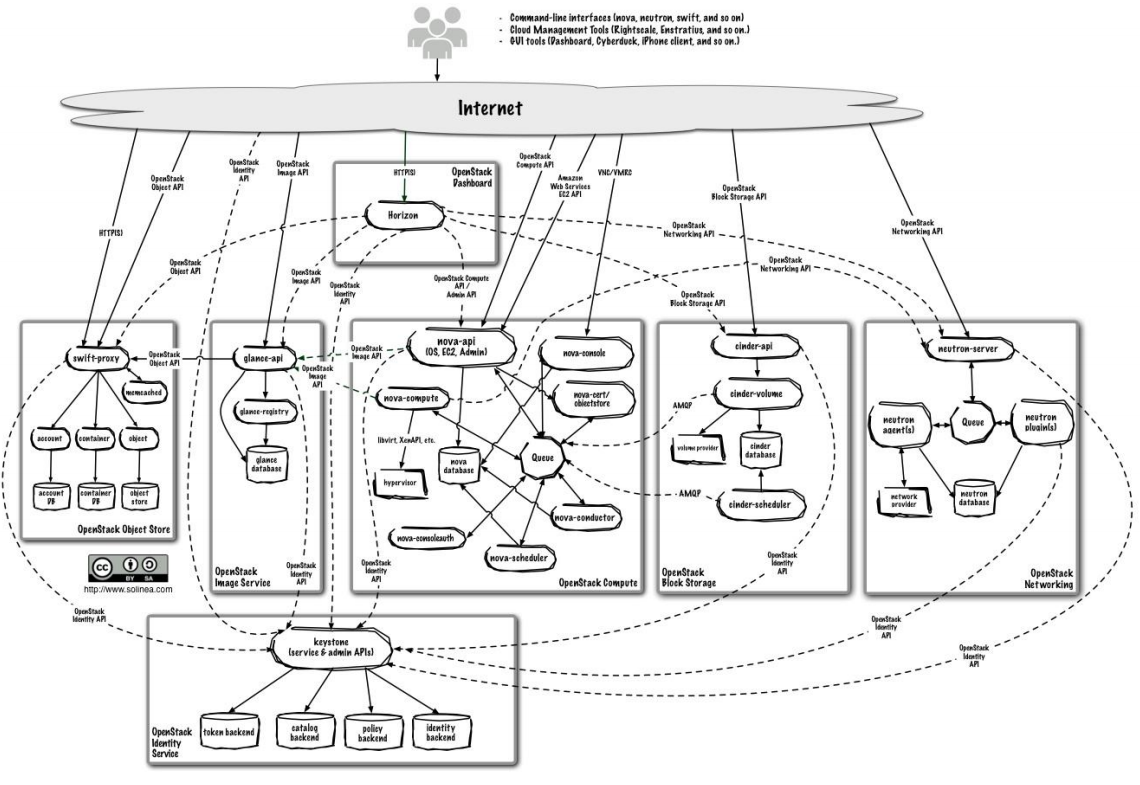
\includegraphics[width=0.8\linewidth]{images/spagetti.png}
	\end{figure}
\end{frame}

\begin{frame}
	\frametitle{Really???}
	\begin{figure}
		
\includegraphics[width=0.8\linewidth]{images/jc.jpg}
	\end{figure}
\end{frame}

\subsection{Organization} 
\begin{frame}
	\frametitle{A simpler view}
	\begin{figure}
		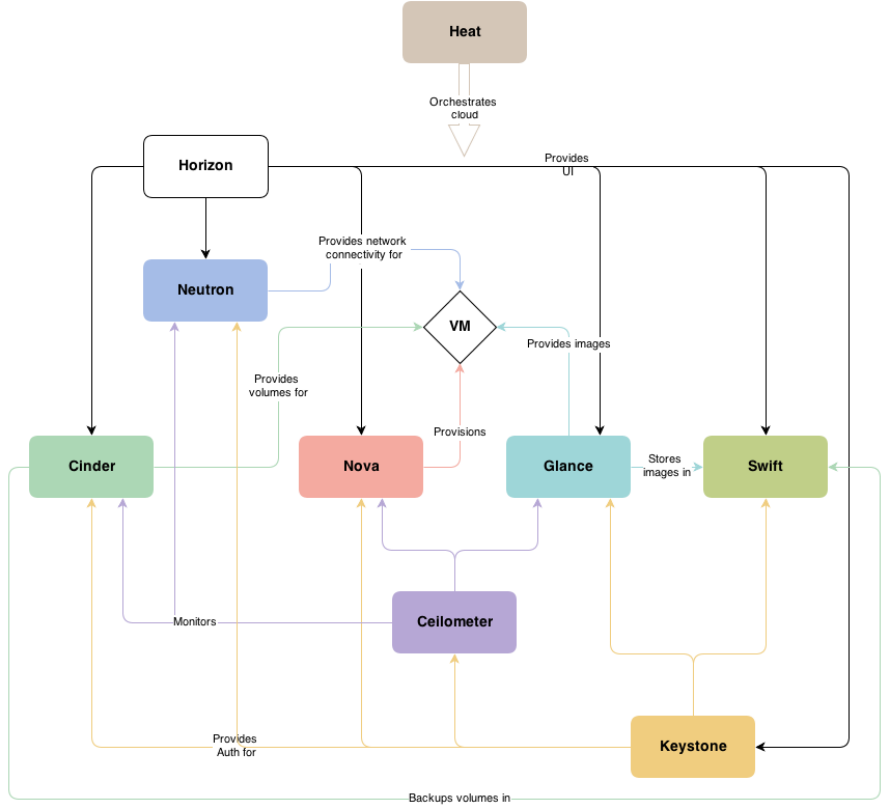
\includegraphics[width=0.7\linewidth]{images/diagram.png}
	\end{figure}
\end{frame}

\begin{frame}
	\frametitle{Installers}
	\begin{itemize}
		\item TripleO/OSP
		\item Packstack
		\item Fuel
	\end{itemize}
\end{frame}
